\section{Repository analysis} \label{repo_analysis}

This thesis comprises the documents on the repositories of the \acrshort{tu}, \acrshort{hu} and \acrshort{fu}. The repositories are called depositonce, edoc and refubium, respectively. There are 62,507 documents\footnote{As of 26/05/2021.} among the three repositories. As mentioned in section \ref{problem_scope_docs}, we are only interested in theses and publications written in English. We thus discard documents referring to research data, university related documents and others, leaving us with 29,399 documents, with 47 \% of them belonging to refubium and 63 \% being publications. The analysis presented in this chapter only considers these relevant documents.

We start by exploring the existing subjects in section \ref{repo_analysis_subjects}, which are at the core of this thesis. 81 \% of them appear in only one document, and only 5 \% in more than three, which renders them useless for navigating the repositories. We also present the distribution of the \acrfull{ddc} subjects. \textit{Science}, \textit{Social Sciences} and \textit{Technology} cover 83 \% of all the relevant documents.

We then look at venues (section \ref{repo_analysis_venues}) and contributors (section \ref{repo_analysis_contributors}), which are also useful to relate documents to one another. Venues are assigned to four documents on average, and only 2 \% of the publications don't have one. Referees and advisors, which we will use as a replacement for venues when considering theses, also offer a good coverage of the theses, with all but 4 \% of the theses having an advisor or a referee.

Finally, in section \ref{repo_analysis_data}, we analyze the actual data that will be used to perform \acrshort{si}: the titles and abstracts of the documents. All documents in the repositories are required to have a title, so all the documents have one. Abstracts, on the other hand, are optional. 6 \% of the relevant documents don't have one. In this final section, we also discuss how certain titles and abstracts are tagged as being written in English when they are not. When running a language detection algorithm, we find out that 320 abstracts are not actually written in English. We try to solve this issue for detecting the language of the other abstracts of the documents, which are tagged as being written in other languages.

\subsubsection{Set of subjects} \label{problem_scope_subjects}

Our dataset comprises considerably fewer documents than \acrshort{mag} (tens of thousands instead of hundreds of millions). Given that our goal is to relate documents to one another through their content, and we are focusing on small repositories, we don't require such granular subjects. If we used all the \acrshort{mag} subjects, most of them would be left unassigned, and many others would be assigned only once. We therefore pick a subset of these subjects.

\acrshort{mag} structures their set of subject as a hierarchy, where the first level comprises 19 subjects, which we call fields for clarity. Under each field, there exist five further hierarchy levels. We extract the subjects from OpenAlex, which is currently the best data source for subjects and publications of \acrshort{mag} (see section \ref{mag_access_data}).

In section \ref{problem_scope_subjects_retrieve}, we present our subject retrieval procedure. We discuss how many subjects we retrieve per field, and on what conditions we pick among the thousands of candidates. Then, we present the resulting set of subjects in section \ref{problem_scope_subjects_result}.

\paragraph{Subject retrieval} \mbox{} \label{problem_scope_subjects_retrieve}

We have extracted up to 200 descendants of each of the 19 fields. We consider how many publications a subject has been assigned to, assuming that popular subjects are more likely to appear in the repositories. We have tried different thresholds for how many assignments a subject needs to be considered, to strike a balance between picking subjects from the upper levels, which are more general, and picking subjects that are popular.

The problem is that the fields differ in popularity. For example, \textit{Medicine} has more than 200 subjects in the third level with more than 25k works, whereas \textit{Environmental science} only has 31 across all levels. We therefore start with a larger limit, iterate over all levels and all fields, and decrease the limit before iterating again. We first iterate through the descendants of each field and add subjects that are assigned to at least 25,000 publications. If the list of a field does not include 200 subjects after this iteration, we do so again, considering subjects assigned to at least 10,000. We repeat this procedure with 5,000, 1,000 and 100 assignments. When we iterate through the subjects of a field, we start by the second level and descend if necessary.

To avoid uninformative Wikipedia texts such as ``Emotionalism may refer to:'', we discard subjects whose description says ``Wikimedia disambiguation page'' or ``Wikimedia glossary list article''. The description from a subject comes from the corresponding Wikidata link, through which we later extract the Wikipedia link. For each subject that meets these requirements, we append it to all the fields it has in its list of ancestors, to keep the number of subjects as low as possible while providing good coverage of the fields.

\paragraph{Resulting set of subjects} \mbox{} \label{problem_scope_subjects_result}

\begin{figure}
    \centering
    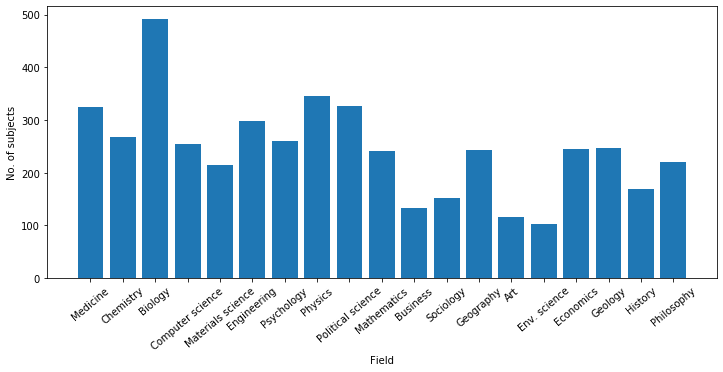
\includegraphics[width=\textwidth]{figures/unsupervised_approach/subjects_per_field.png}
    \caption{Number of subject that descend of each of the fields.}
    \label{fig:subjects_per_field}
\end{figure}

2,157 subjects were extracted with this procedure, which results on an average of 114 subjects per field. We could extract 200 subjects for all fields except for \textit{Environmental Science}, \textit{Business}, \textit{Sociology}, \textit{Art} and \textit{History}. On the other hand, \textit{Medicine}, \textit{Biology} and \textit{Physics} have more than 300 descendant subjects under the ones we have collected. This is because subjects can descend from multiple fields. For example, \textit{Neuroscience} can be classified under \textit{Biology}, \textit{Medicine} and \textit{Computer science}. The number of subjects per field can be seen in figure \ref{fig:subjects_per_field}.

All 25 subjects of the second level have been picked, followed by 1,999 of the third level, 108 of the fourth, and 6 of the fifth. On average, subjects are assigned to 197,180 publications. No subjects are assigned to less than 100 documents, as this was a requirement in the extraction procedure. Regarding the hierarchy of the subjects, all but 13 of them have ancestors in all levels above them. Two subjects of the third, \textit{Sensitivity} and \textit{Boundary}, are directly linked to fields. \textit{Sensitivity} is a descendant of both \textit{Engineering} and \textit{Mathematics}, whereas \textit{Boundary} descends from \textit{Mathematics}. The remaining eleven subjects that don't have ancestors in all previous levels belong to the fourth level. All of them descend from subjects of the second level, thus skipping the third level.
\subsection{Publishing venues} \label{repo_analysis_venues}

The venue where a publication was published is important information that relates documents to one another regarding the topics they discuss. For example, the publishing venue of an article is a journal. Theses don't have publishing venues, as they serve another purpose (namely, evaluating the student's knowledge and ability). In this section, we discuss the publishing venue for each type of document. Given that how the venue is stored differs depending on the repository, we look at each of them separately.

Table \ref{tab:publishing_venues} shows the most common field names per publication type and repository. For example, all 3,233 articles present in depositonce have the name of the journal they were published in stored in a field called \textit{``journalTitle''}. Books in refubium often have two fields named \textit{``series''}, one for the name of the series and the other for the issue number that corresponds to the book.

The most popular venue is called ``Sonderforschungsbereich 649: Ökonomisches Risiko'' which appears on 809 publications of edoc. The second most popular venue is also a ``Sonderforschungsbereich'' of the \acrshort{hu} (which means ``research area in English'') and it appears in 583 publications. The third one is the first real publishing venue: ``PLoS ONE'', with 533 publications.

On average, venues appear on 4.2 publications. There are 4,418 venues present across all three repositories, 2,867 of which (65 \%) are only assigned to one publication. From this follows that 2,867 publications (15 \%) have a venue which they don't share with any other publication. As shown in figure \ref{fig:pubs_venue_alone}, more than half of these publications belong to refubium. Furthermore, 292 publications (2 \%) don't have a venue, almost half of them belonging to depositonce. The amount of these publications that belong to each repository is illustrated in figure \ref{fig:pubs_with_no_venue}.

\begin{table}
\centering
\begin{tabular}{|c|c|c|c|c|}
\hline
\thead{Doc. type} & \thead{Repository} & \thead{\# docs} & \thead{Field name} & \thead{\# fields} \\
\hline\hline
\multirow{3}{*}{Article} & depositonce & 3233 & journalTitle & 3233 \\ \cline{2-5}
& edoc & 1904 & container-title & 1846 \\ \cline{2-5}
& refubium & 7519 & journalTitle & 3517 \\ \cline{2-5}
\hline
\multirow{3}{*}{Book part} & depositonce & 155 & bookTitle & 155 \\ \cline{2-5}
& edoc & 160 & container-title & 214 \\ \cline{2-5}
& refubium & 172 & bookTitle & 109 \\ \cline{2-5}
\hline
\multirow{3}{*}{Book} & depositonce & 91 & series & 118 \\ \cline{2-5}
& edoc & 2128 & container-title & 2076 \\ \cline{2-5}
& refubium & 1184 & series & 2211 \\ \cline{2-5}
\hline
\multirow{3}{*}{Conference Obj.} & depositonce & 465 & series & 450 \\ \cline{2-5}
& edoc & 489 & container-title & 993 \\ \cline{2-5}
& refubium & 378 & series & 0 \\ \cline{2-5}
\hline
\end{tabular}
\caption{Field names where the publishing venues are stored per document type and repository.}
\label{tab:publishing_venues}
\end{table}

\begin{figure}
  \begin{subfigure}[t]{0.45\textwidth}
    \centering
    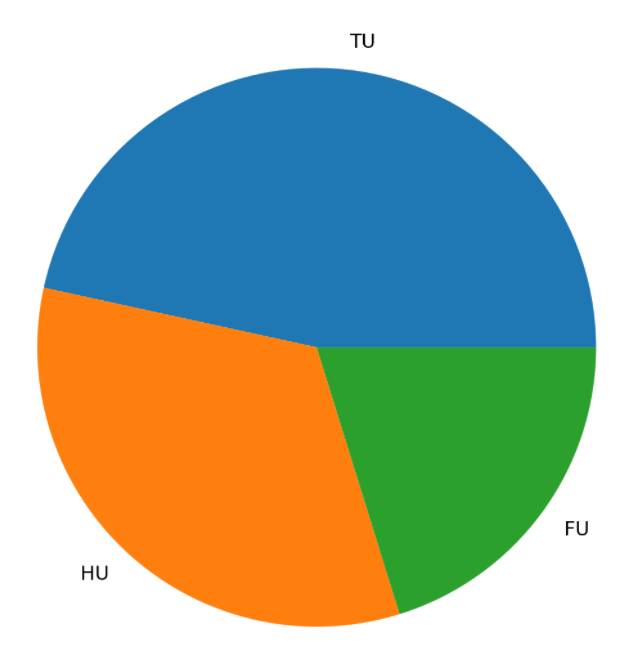
\includegraphics[width=\textwidth]{figures/repository_analysis/pubs_with_no_venue.PNG}
    \caption{Publications with no venue}
    \label{fig:pubs_with_no_venue}
  \end{subfigure}
  \hfill
  \begin{subfigure}[t]{0.41\textwidth}
    \centering
    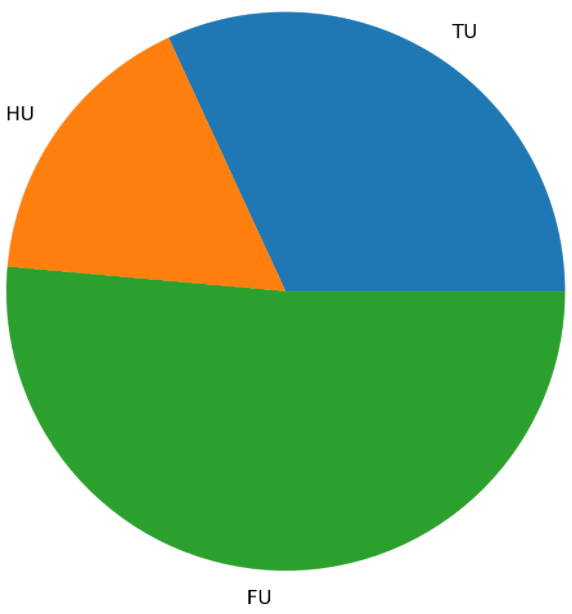
\includegraphics[width=\textwidth]{figures/repository_analysis/pubs_venue_alone.PNG}
    \caption{Publications that don't share the venue with any other publication.}
    \label{fig:pubs_venue_alone}
  \end{subfigure}
  \caption{Pie charts about the venues of the publications.}
\end{figure}
\subsection{Contributors} \label{repo_analysis_contributors}

\begin{figure}
    \centering
    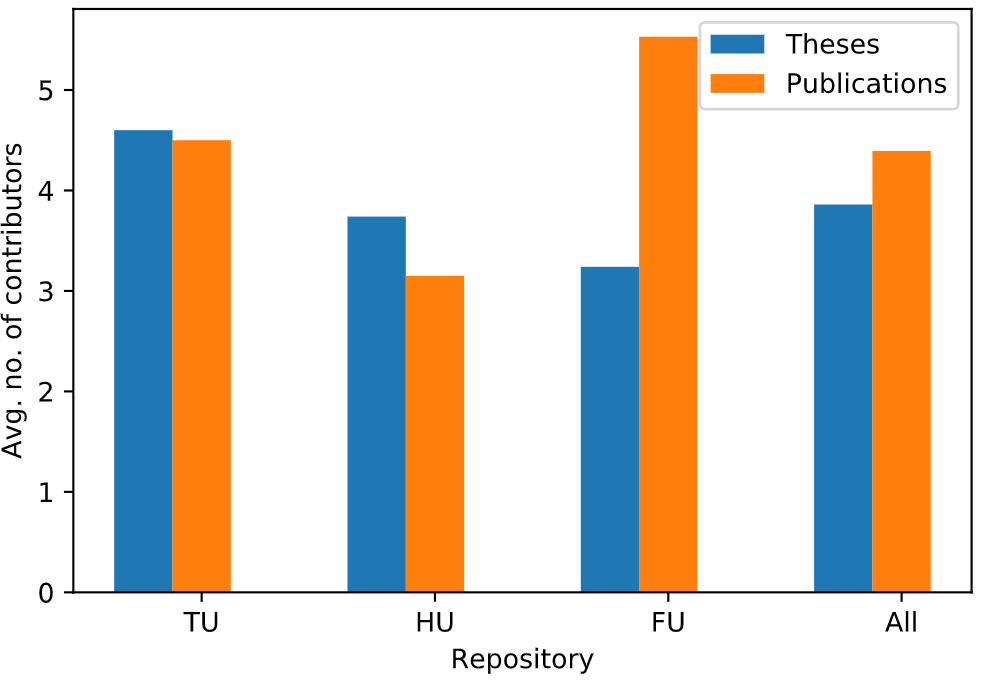
\includegraphics[width=.7\textwidth]{figures/repository_analysis/avg_contributors.PNG}
    \caption{Avg. number of contributors per document type and repository.}
    \label{fig:avg_contributors}
\end{figure}

In this section, we look at what types of contributors are present in the repositories and how often they occur. On average, documents of depositonce, edoc and refubium have 4.5, 3.4 and 4.7 contributors, respectively. In depositonce, publications and theses offer similar average numbers of contributors. In edoc, there are 0.5 more contributors in theses than in publications. In refubium it is the other way around: publications have 2.3 more contributors than theses on average. These numbers are shown illustrated in figure \ref{fig:avg_contributors}.

Regarding the types of contributors, publications usually include only the author. Edoc includes a significant number of editors, as shown in figure \ref{fig:author_types}. Theses, on the other hand, have other important types of authors: referees and advisors. After analyzing the authors, we will look at these two author types in the following sections. They are relevant because they could be used to relate documents, the same role that venues play for publications.

\begin{figure}
    \centering
    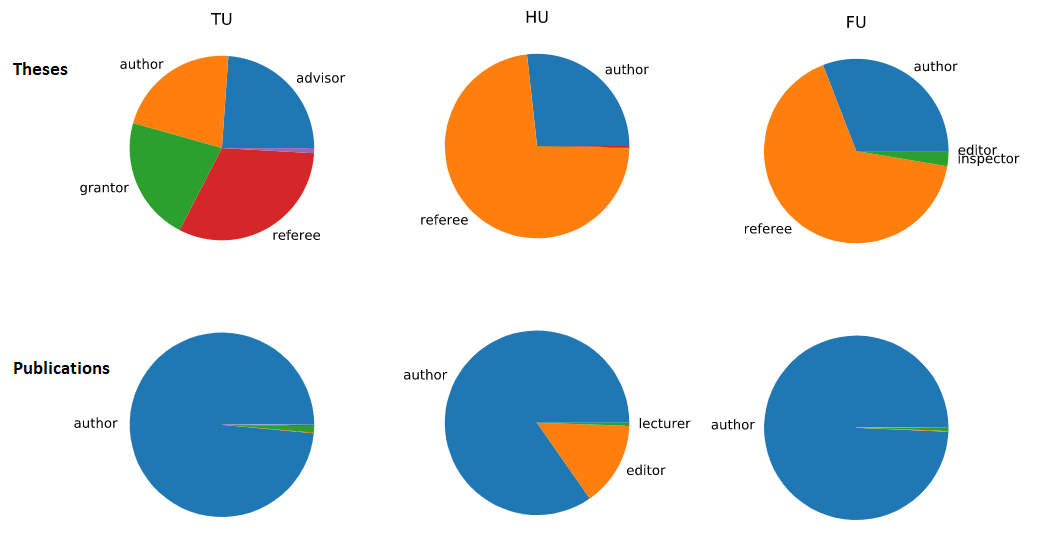
\includegraphics[width=\textwidth]{figures/repository_analysis/author_types_pretty.png}
    \caption{Author types that appear on each repository depending on the document type.}
    \label{fig:author_types}
\end{figure}


\subsubsection{Authors}

Authors are the most important contributors, as they are responsible for the content of the document. Only 207 out of the 29,399 documents don't have an author (0.7 \%), all of them being publications and 144 of them belonging to refubium. Publications have on average more authors than theses. Out of all 10,773 theses, only two of them have more than 1 author. Both of them belong to edoc. In contrast, 80 \% of the publications have multiple authors. This difference is expected, as students are usually required to write a thesis by themselves, whereas researchers often collaborate and publish their work together.

Authors of theses rarely have more than one thesis, as shown in figure \ref{fig:n_publications_per_author}. In total, 56 alumni have authored multiple theses. The real number is lower, as a quick check of some of them reveals the existence of duplicates. The ones that do have two theses to their name are Master's students that went on to pursue a PhD. On the other hand, the researchers present in the repositories have authored on average 1.6 publications. The two researchers with the most publications are Kai Nagel, from the \acrshort{tu} Berlin, and Wolfgang Härdle, from the \acrshort{hu} Berlin. Both have authored 143 publications. Still, more than 77 \% of the researchers have authored only one publication. Figure \ref{fig:n_publications_per_author} shows the distribution of researchers among the number of publications they have authored.

\begin{figure}
    \centering
    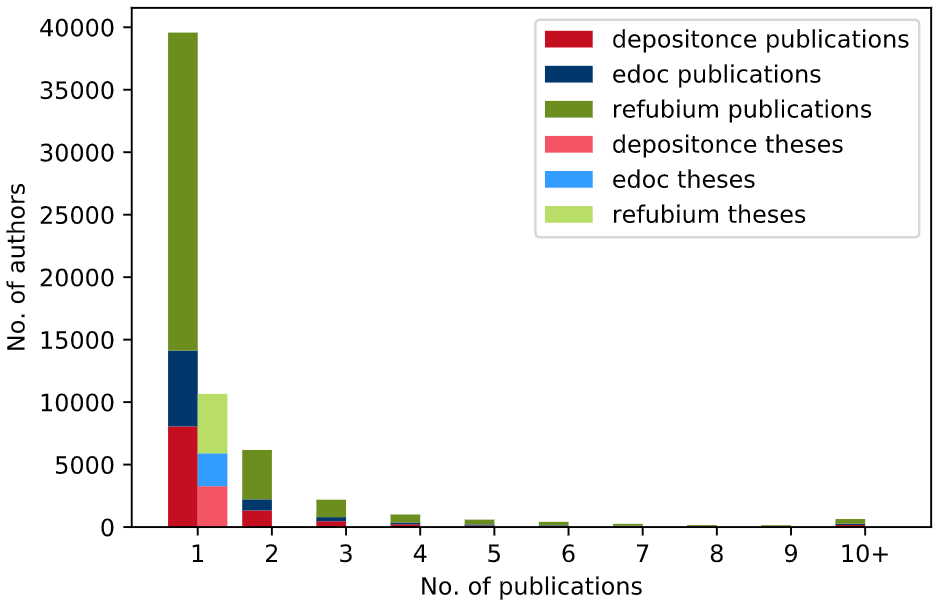
\includegraphics[width=.7\textwidth]{figures/repository_analysis/n_publications_per_author.PNG}
    \caption{No. of authors per no. of publications.}
    \label{fig:n_publications_per_author}
\end{figure}


\subsubsection{Referees}

Referees are in charge of evaluating the student's work and assigning a grade to the submitted thesis. Thus, every thesis requires at least one referee. Both edoc and refubium provide referees for almost all their theses. Only 39 and 41 documents are missing a referee, respectively. On the other hand, 1,442 theses of depositonce do not include a referee, which amounts to 19 \% of all theses.  These and all other facts presented in this section are summarized in table \ref{tab:referees}.

A caveat to the referees of refubium is the presence of ``N.N.'' as the most popular referee, appearing 1,126 times. It stands for the Latin phrase \textit{Nomen Nescio}, which means ``unknown person''. Therefore, all theses of refubium that include ``N.N.'' or variations of it can also be seen as theses without a referee. Then, refubium has 662 theses without a referee instead of 41, which amounts to 5 \% of all its theses. In total, depositonce comprises 4,780 referees, 2,388 of which are distinct. In edoc there are 7,289 referees, of which 3,390 are distinct. In refubium there are 9,133 referees and 4,863 distinct ones.

The documents that do have a referee often include more than two. On average, theses in depositonce include 2.6 referees, those of edoc 2.8 and those of refubium 2.2. Please note that theses averages don't take into account theses that have zero referees. The \textit{Nomen Nescio} referees of refubium are also ignored. The referees are professors of the universities and therefore appear frequently on the repositories, as they evaluate numerous theses. On average, professors appear two times in the repositories as referees. In depositonce there are 57 referees who have evaluated more than ten theses; in edoc there are 97 such referees and in refubium, 88. The most recurrent referees of each repository are Rupert Mutzel (FU Berlin), who has been a referee for 72 theses Wolfgang Härdle (HU Berlin), who appears on 60 theses and Peter Neubauer (TU Berlin), who appears on 45 theses.

\begin{table}[]
    \centering
    \begin{tabular}{|c|c|c|c|c|}
    \hline
         \thead{Repository} & \thead{\# referees} & \thead{\# distinct  \\ referees} & \thead{Avg. \# \\ referees \\ per thesis} & \thead{\# theses \\ without \\ a referee} \\
         \hline
         depositonce & 4,780 & 2,338 & 2.6 & 1442 (19 \%) \\
         \hline
         edoc & 7,289 & 3,390 & 2.8 & 39 (1 \%) \\
         \hline
         refubium & 9,133 & 4,863 & 2.2 & 662 (5 \%) \\
         \hline
    \end{tabular}
    \caption{Facts regarding the referees of theses.}
    \label{tab:referees}
\end{table}

\subsubsection{Advisors}

Advisors are also a building block of a thesis. They are experts on the topics handled by the thesis they advise on, and also help the student with the writing process. All facts presented in this section are summarized in table \ref{tab:advisors}. Only depositonce has a maintained list of advisors. All but 124 theses (4 \% of all theses) have at least one advisor. edoc only has 13 advisors and refubium has none. Coincidentally, depositonce is the repository where the referees are not as well maintained as in the other repositories. It seems that users of depositonce care more about advisors, and users of edoc and refubium about referees.

Students usually have just one advisor. In depositonce, theses include on average 1.1 advisors; in edoc, 1.3 advisors. Regarding how many theses share the same advisor, the average for depositonce is 3.3 theses per advisor. For edoc, the average is 1.5. Depositonce has 84 advisors that appear on more than ten different theses. edoc, on the other hand, has none. The advisor of depositonce with the most theses is Klaus-Robert Müller, who has advised 47 theses. For edoc, the most recurrent advisor is Wolfgang Härdle, who has advised 6 theses.

\begin{table}
    \centering
    \begin{tabular}{|c|c|c|c|c|}
    \hline
         \thead{Repository} & \thead{\# advisors} & \thead{\# distinct  \\ advisors} & \thead{Avg. \# \\ advisors \\ per thesis} & \thead{\# theses \\ without \\ an advisor} \\
         \hline
         depositonce & 3,603 & 1,080 & 1.1 & 124 (4 \%) \\
         \hline
         edoc & 19 & 13 & 1.3 & 2,659 (99 \%) \\
         \hline
         refubium & 0 & 0 & 0 & 4,815 (100 \%) \\
         \hline
    \end{tabular}
    \caption{Facts regarding the advisors of theses.}
    \label{tab:advisors}
\end{table}

\subsection{Titles and abstracts} \label{repo_analysis_data}

As mentioned in the introduction, we consider the titles and abstracts of the documents to represent them. In this section, we will present some facts about these two fields, regarding how often they are left empty in the repositories and other noise factors in our corpus, such as the hundreds of texts that are tagged as being written in English when they are not.

\subsubsection{Fill quota}

The title is a required field in all three repositories and is therefore present for all the documents of our corpus. Abstracts, on the other hand, are optional fields. It is empty in 135 of the 7,438 documents of depositonce (1.8 \%), in 922 of the 7,497 documents of edoc (12.3 \%) and in 776 of the 14,464 documents of refubium (5.4 \%). In total, 1,833 of 29,399 documents (6.2 \%) don't have an abstract. Most of the documents that are missing the abstract are publications. None of the 135 documents of depositonce that don't have an abstract are theses. In edoc, only 25 of the 922 documents (2.7 \%) without an abstract are theses; in refubium, 11 of 765 (1.4 \%).

\subsubsection{Foreign languages}

Looking at the data reveals that there are several titles and abstracts which should be written in English (as stated in the tags of the field) but are actually in German. This is the case for 678 titles (2.3 \% of all titles) and 320 abstracts (1.1 \%). Out of the 678 titles, 542 are written in German (80 \%). 381 of these belong to refubium, 90 to depositonce and 71 to edoc. Some titles included in this list are actually in English, but have been misclassified due to their brevity. For example, the two titles that are considered to be written in Polish are ``Przy Bazantarni, Warsaw'' and ``Democrazy ?!''. The second one is clearly not Polish, but given that the word ``Democrazy'' ends like ``Przy'', a misclassification can happen.

Detecting the language of the abstracts is more reliable given the larger size of the text. Out of the 320 abstracts that are not written in English, 319 of them are in German and 1 in Polish. Again, many of the abstracts that are considered to be written neither in German nor English are often in English, but misclassified due to their brevity.

The difference in length between texts written in German and those written in other languages (excluding English) is illustrated in figure \ref{fig:foreign_languages}. German titles comprise 85 characters on average, whereas those in other languages comprise 18 characters. The difference is even more clear when looking at abstracts: German abstracts are 2,682 characters long on average, and those in other languages only 965 characters long. This difference in length supports our hypothesis that texts that are classified as other languages other than German are often errors that occur because of the brevity of the text.

\begin{figure}
    \centering
    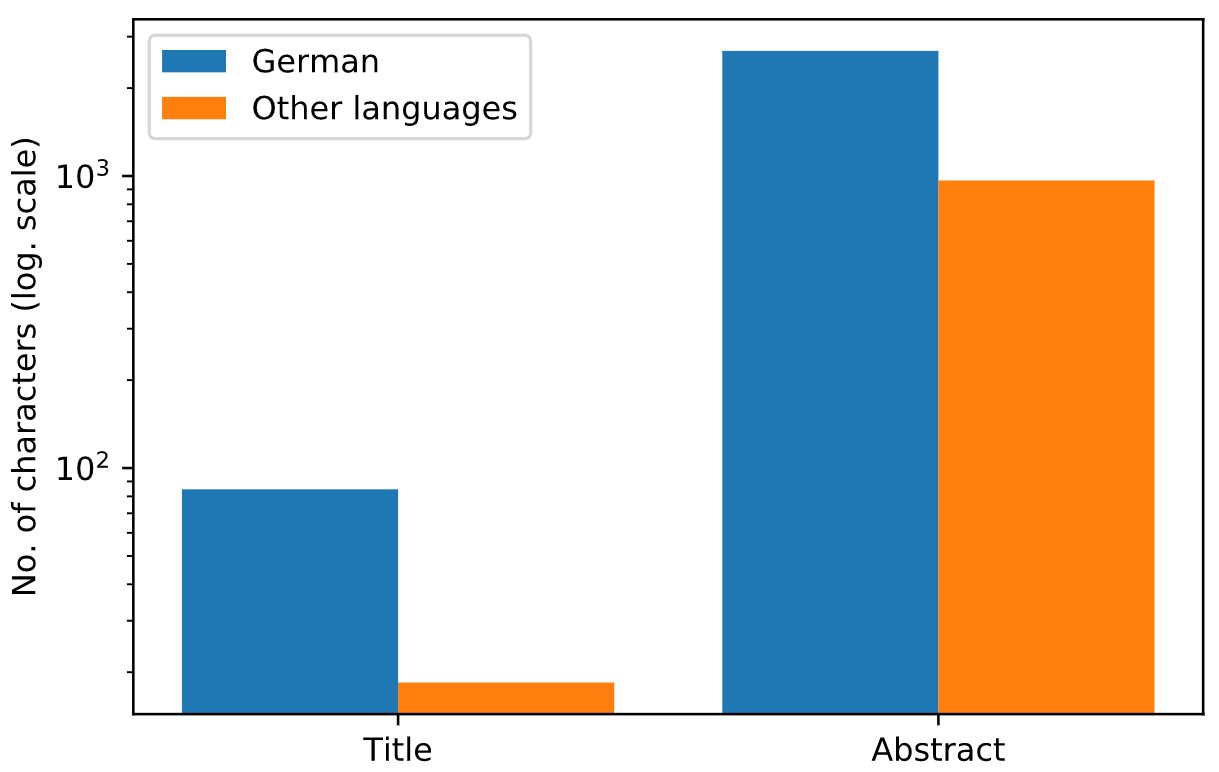
\includegraphics[width=.7\textwidth]{figures/repository_analysis/foreign_languages.PNG}
    \caption{Lengths of titles and abstracts that are not written in English.}
    \label{fig:foreign_languages}
\end{figure}

We determined the language of the texts using the Python package \textit{langdetect}\footnote{\url{https://github.com/Mimino666/langdetect}}, which uses a naive Bayes filter to identify the most probable language out of 53 options. We run the function \textit{detect\_langs} 10 times for each text: a text is written in a foreign language if the probability of the first result is always above 99 \% and the language remains the same throughout all 10 executions. We then use langdetect again to retrieve English texts from the repositories that have been tagged incorrectly (e.g. English texts where the language is said to be German). After extracting all titles and abstracts of each document, we run the language detection procedure described above for each of the possibilities and return the one in English, if any.

Doing so returns English titles for 443 out of the 678 documents (65 \%) with titles in foreign languages and English abstracts for 306 out of the 320 documents (96 \%). When looking at the tags of these retrieved fields, we see that most of them incorrectly state that the text is in German. This is the case for 274 out of the 306 found abstracts. We then run the language detection procedure one again on the improved data. Although we expect to encounter more texts in English, we cannot assume that the number of English texts is now the number of English texts in the original data minus the number of the English texts retrieved with the language detection procedure because of the randomness of the detection model.

This final run shows that 271 titles  (0.9 \%) and 14 abstracts (0.04 \%) are written in foreign languages. 177 of the 271 titles (65 \%) in foreign languages are in German, and all abstracts but one (which is written in Polish) are in German. With this language detection procedure, we have been able to improve the quality of our data, reducing the number of texts written in foreign languages. We have retrieved English texts for 409 titles and 306 abstracts that were previously in foreign languages because of incorrect language tags in the data. 

Please note that these numbers are not fully reliable, given that the model is not always able to correctly predict the language of a text. This can be seen in the number of titles that were deemed to be in foreign languages when looking for alternative titles and those detected in the final run. The first round showed that 235 titles were in foreign languages. Running the same detection procedure again output 271 titles. On the other hand, the detected language for the abstracts remained the same in both runs. This shows that the length of the text is an important factor when evaluating the performance of the language detection model.
